\documentclass[tikz,border=8pt]{standalone}
% Shared look for every TikZ diagram. Load with \input{../../tools/tikz-style.tex}
\usepackage[T1]{fontenc}
\usepackage{lmodern}
\renewcommand{\sfdefault}{lmr}  % diagrams use the same serif as the text
\usetikzlibrary{arrows.meta, positioning, shapes.geometric, calc, fit, backgrounds}
\definecolor{cblue}{HTML}{4C78A8}
\definecolor{corange}{HTML}{F58518}
\definecolor{cgreen}{HTML}{54A24B}
\definecolor{cred}{HTML}{E45756}
\definecolor{cpurple}{HTML}{B279A2}
\definecolor{cgrey}{HTML}{6B6B6B}
\tikzset{
  every picture/.style={font=\sffamily, line width=1.2pt},
  box/.style={draw=#1, fill=#1!12, rounded corners=4pt, align=center, inner sep=7pt, minimum height=1.1cm},
  box/.default=cgrey,
  arrow/.style={-{Stealth[length=3mm]}, draw=cgrey, line width=1.4pt},
  title/.style={font=\sffamily\bfseries\Large},
  note/.style={font=\sffamily\small, text=cgrey, align=center},
}
\AtBeginDocument{\hyphenpenalty=10000 \exhyphenpenalty=10000}

\begin{document}
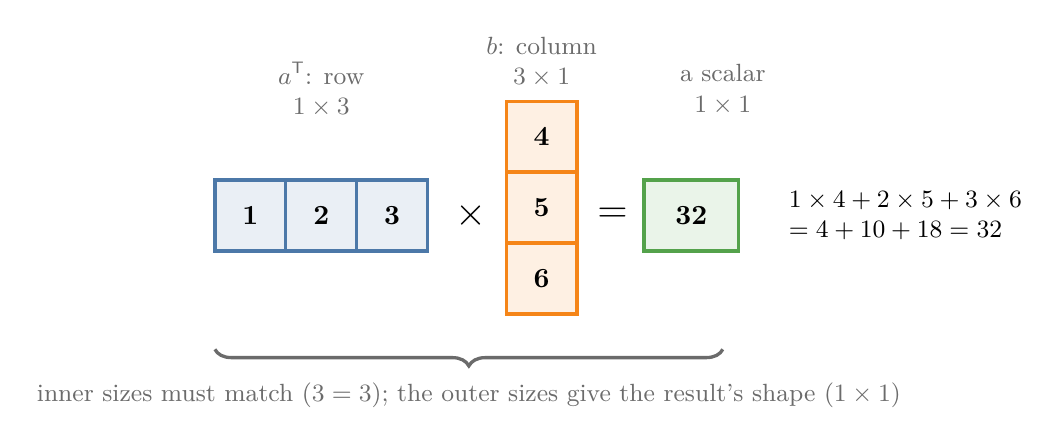
\begin{tikzpicture}[c/.style={draw=#1, fill=#1!12, minimum size=0.9cm, font=\bfseries}]
  % row a^T
  \foreach \v [count=\i] in {1,2,3} \node[c=cblue] (r\i) at (\i*0.9,0) {\v};
  \node[note] at (1.8,1.6) {$a^{\mathsf T}$: row\\ $1 \times 3$};
  \node at (3.7,0) {\Large $\times$};
  % column b
  \foreach \v [count=\i] in {4,5,6} \node[c=corange] (k\i) at (4.6,1.9-\i*0.9) {\v};
  \node[note] at (4.6,1.95) {$b$: column\\ $3 \times 1$};
  \node at (5.5,0) {\Large $=$};
  \node[c=cgreen, minimum width=1.2cm] (res) at (6.5,0) {32};
  \node[note] at (6.9,1.6) {a scalar\\ $1 \times 1$};
  \node[font=\small, align=left, anchor=west] at (7.6,0) {$1\times4 + 2\times5 + 3\times6$\\ $= 4 + 10 + 18 = 32$};
  \draw[decorate, decoration={brace, mirror, amplitude=6pt}, cgrey] (0.45,-1.7) -- (6.9,-1.7)
     node[midway, below=8pt, note] {inner sizes must match ($3 = 3$); the outer sizes give the result's shape ($1 \times 1$)};
\end{tikzpicture}
\end{document}
